\documentclass[a4paper,11pt]{article}
\usepackage[T1]{fontenc}
\usepackage[utf8]{inputenc}
\usepackage{lmodern}
\usepackage[spanish]{babel}
\usepackage{graphicx}
\usepackage{float}
%\usepackage{biblatex}
%\usepackage{url}
\usepackage{hyperref}

\title{Monitor de Sistema}
\author{Aguilar Enriquez, Paul Sebastian a.k.a Penserbjorne}

\begin{document}

\maketitle
\tableofcontents

\begin{abstract}
\textbf{Planteamiento del profesor:} Programar un monitor de recursos del sistema operativo (de los recursos que juzguen útiles, interesantes, o que decidan por la razón que sea), pero con la particularidad o requisito de que
debe trabajar de forma concurrente, sincronizando multihilos, multiprocesos o ambos. Empleen los mecanismos de sincronización que consideren adecuados.

\textbf{Propuesta del alumno:} Diseñar e implementar un monitor de (algún/algunos) recurso/recursos del sistema, en este caso se pretende realizar para la plataforma GNU/Linux ...
\end{abstract}

\section{Monitor de Sistema}

Investigando un poco, sobre todo por Internet, es muy complicado encontrar una definicion exacta de lo que es un ''Monitor de Sistema''. Para el usuario intermedio-avanzado de un equipo de computo puede que el termino sea inherente, sin embargo a continuacion dejaremos algunas definiciones que podrian describir un poco lo que es un ''Monitor de Sistema''.

\begin{enumerate}
  \item El monitor del sistema muestra qué programas están en ejecución y cuánto procesador, tiempo, memoria y espacio en disco están usando.\cite{ref:web1}
  
  \item ... es una aplicación integrada en los sistemas operativos ... , gracias a la cual podremos obtener información de los programas y procesos que se ejecutan en el equipo, además de proporcionar los indicadores de rendimientos más utilizados en el equipo.\cite{ref:web2}
  
  \item These tools are primarily divided into two main categories: real time and log-based. Real time monitoring tools are concerned with measuring the current system state and provide up to date information about the system performance. Log-based monitoring tools record system performance information for post-processing and analysis and to find trends in the system performance.\cite{ref:web3}
  
  \item Los procesos que se muestran ... pueden ser apps del usuario, apps del sistema utilizadas o procesos invisibles en segundo plano.\cite{ref:web4}

\end{enumerate}

En general podriamos resumir que un ''Monitor de Sistema'' es un software que monitorea mayormente en tiempo real los procesos e hilos que estan actualmente en ejecucion mostrando usualmente informacion sobre ellos como seria tiempo, memoria y espacio en disco que estan usando, asi como los indicadores de rendimiento mas comunes de un equipo que podrian ser uso de CPU/hardware, memoria, energia, disco y red.

\section{Ejemplos de Monitores de Sistema}

\subsection{Windows}

Administrador de Tareas

\subsection{Mac OS X}

\cite{ref:web4} El Monitor de Sistema por defecto en Mac OS X es el Monitor de Actividad.\\

Los procesos que se muestran en Monitor de Actividad pueden ser apps del usuario, apps del sistema utilizadas por OS X o procesos invisibles en segundo plano.\\

El Monitor de Actividad permite monitorear cinco aspectos:
\begin{itemize}
  \item CPU
  \item Memoria
  \item Energía
  \item Disco
  \item Red
\end{itemize}

\subsubsection{CPU}

El panel CPU muestra cómo los procesos afectan a la actividad de la CPU (procesador):

\begin{figure}[H]
  \centering
  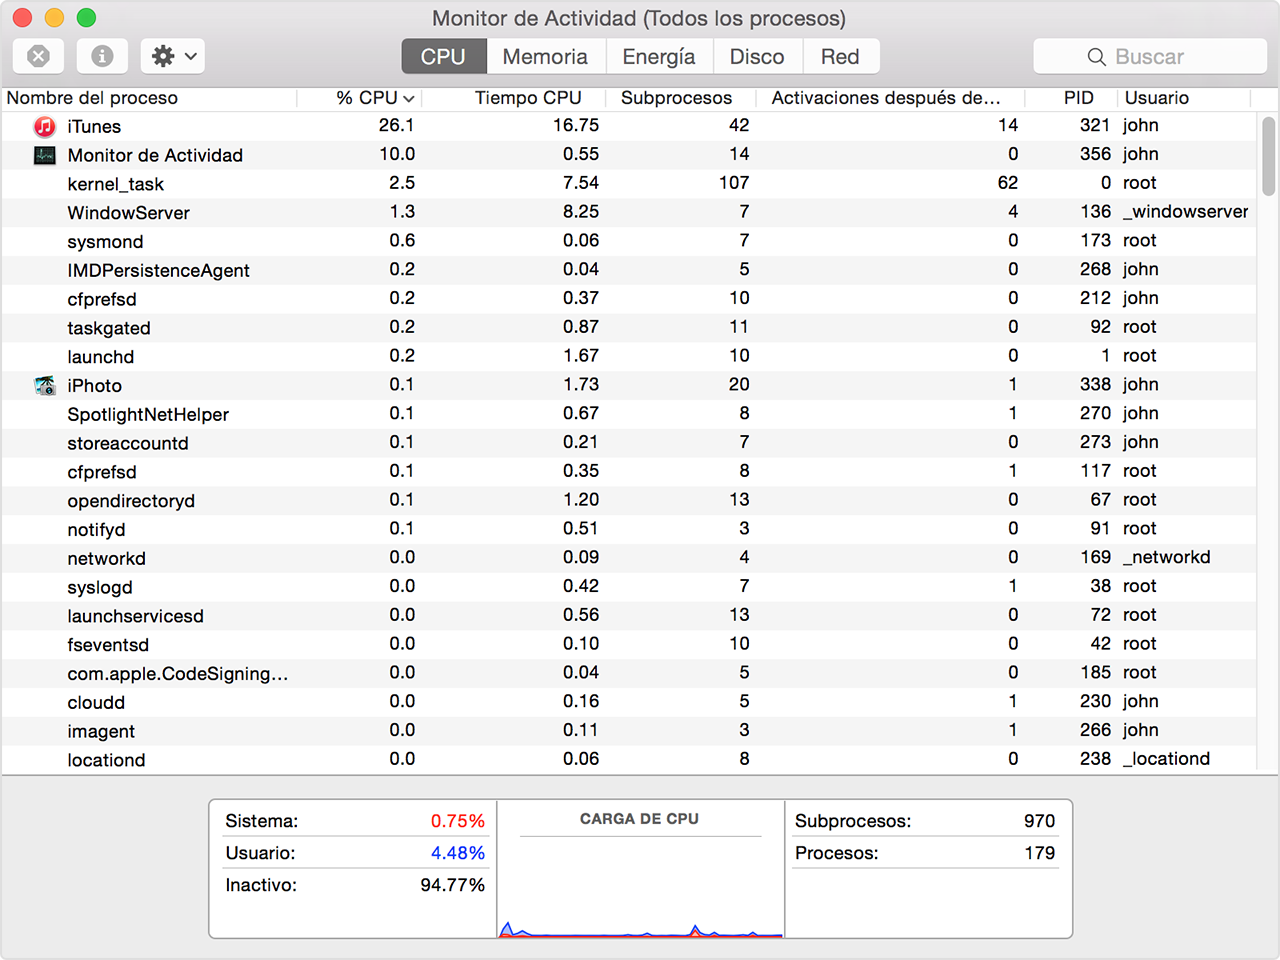
\includegraphics[width=1\textwidth]{01macActivityMonitorCPU}
  \caption{Panel CPU}
  \label{fig:macActivityMonitorCPU}
\end{figure}

En la parte inferior del panel CPU:

\begin{itemize}
  \item \textit{Sistema:} el porcentaje de capacidad de la CPU que utilizan actualmente los procesos del sistema, que son los procesos pertenecientes a OS X.
  \item \textit{Usuario:} el porcentaje de capacidad de la CPU que utilizan actualmente las apps abiertas por el usuario, o los procesos abiertos por esas apps.
  \item \textit{Inactividad:} el porcentaje de capacidad de la CPU que no está en uso.
  \item \textit{Carga de CPU:} el porcentaje de capacidad de la CPU que utilizan todos los procesos del sistema y del usuario. El color azul muestra el porcentaje de capacidad de la CPU total que utilizan actualmente los procesos del usuario. El color rojo muestra el porcentaje de capacidad de la CPU total que utilizan actualmente los procesos del sistema.
  \item \textit{Subprocesos:} la cantidad total de subprocesos utilizados por todos los procesos combinados.
  \item \textit{Procesos:} la cantidad total de procesos que se encuentran en ejecución.

\end{itemize}

\subsubsection{Memoria}

El panel Memoria muestra información acerca de cómo se utiliza la memoria:

\begin{figure}[H]
  \centering
  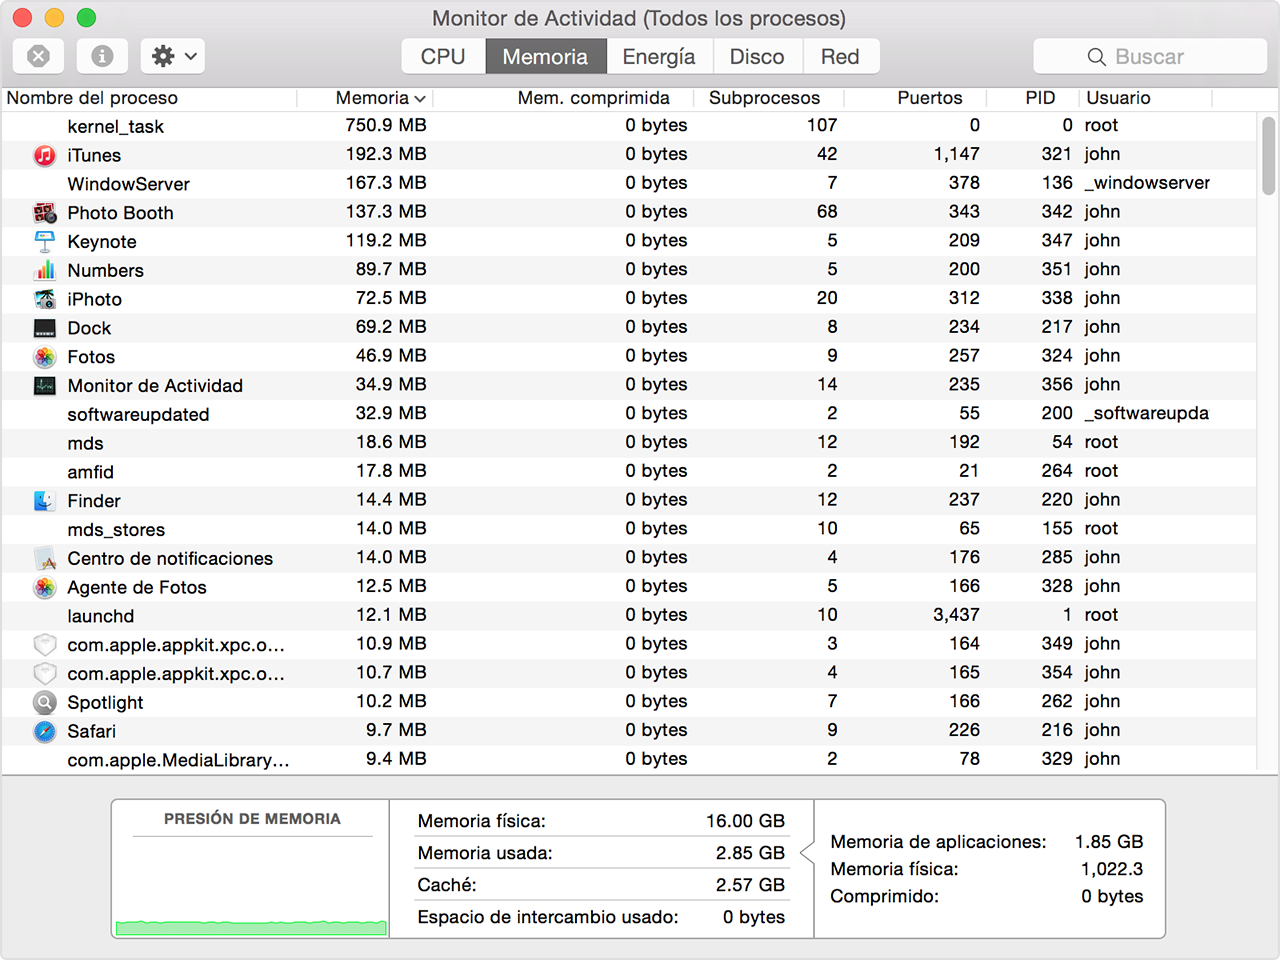
\includegraphics[width=1\textwidth]{02macActivityMonitorMemory}
  \caption{Panel Memoria}
  \label{fig:macActivityMonitorMemory}
\end{figure}

En la parte inferior del panel Memoria:

\begin{itemize}
  \item \textit{Presión de memoria:} el gráfico ayuda a ilustrar la disponibilidad de los recursos de memoria. El estado actual de los recursos de memoria se indica con un color a la derecha del gráfico:   
  \begin{itemize}
    \item \textit{Verde:} los recursos de memoria están disponibles. 
    \item \textit{Amarillo:} los recursos de memoria todavía están disponibles, pero se están utilizando en tareas de procesos de administración de la memoria, por ejemplo, la compresión.
    \item \textit{Rojo:} los recursos de memoria están agotados, y OS X está usando la unidad de arranque como memoria. 
  \end{itemize}
  \item \textit{Memoria física:} la cantidad de RAM instalada en la Mac. 
  \item \textit{Memoria usada:} la cantidad total de memoria usada actualmente por todas las apps y los procesos de OS X.
  \begin{itemize}
    \item \textit{Memoria de aplicaciones:} la cantidad total de memoria usada actualmente por todas las apps y sus procesos.
    \item \textit{Memoria física:} la memoria que no se puede comprimir ni vaciar en la unidad de arranque, es por eso que debe permanecer en la RAM. La memoria física utilizada para un proceso no se puede utilizar para otros procesos. El programador de la app es quien determina la cantidad de memoria física que utilizará una app. 
    \item \textit{Comprimida:} la cantidad de memoria en RAM que se comprime para lograr que haya más memoria RAM disponible para otros procesos.
  \end{itemize}
  \item \textit{Espacio de intercambio usado:} el espacio utilizado en la unidad de arranque para la administración de la memoria de OS X.
  \item \textit{Caché de archivos:} la memoria que usaron recientemente las apps y ahora está disponible para que otras apps la utilicen.

\end{itemize}

\subsubsection{Energia}

El panel Energía muestra el uso general de la energía y la energía usada por cada app:

\begin{itemize}
  \item \textit{Impacto energético:} una medición relativa del consumo de energía actual de la app.
  \item \textit{Impacto energético medio:} el impacto energético medio correspondiente a las últimas ocho horas de funcionamiento de la Mac o al período transcurrido desde el arranque de la Mac, lo que sea más breve. El impacto energético medio también se muestra para las apps que se ejecutaron durante ese período, pero que se cerraron desde entonces.
  \item \textit{App Nap:} las apps que admiten App Nap consumen muy poca energía cuando se encuentran abiertas pero no en uso.
  \item \textit{Evita reposo:} indica si la app está evitando que la Mac entre en reposo.
\end{itemize}

\begin{figure}[H]
  \centering
  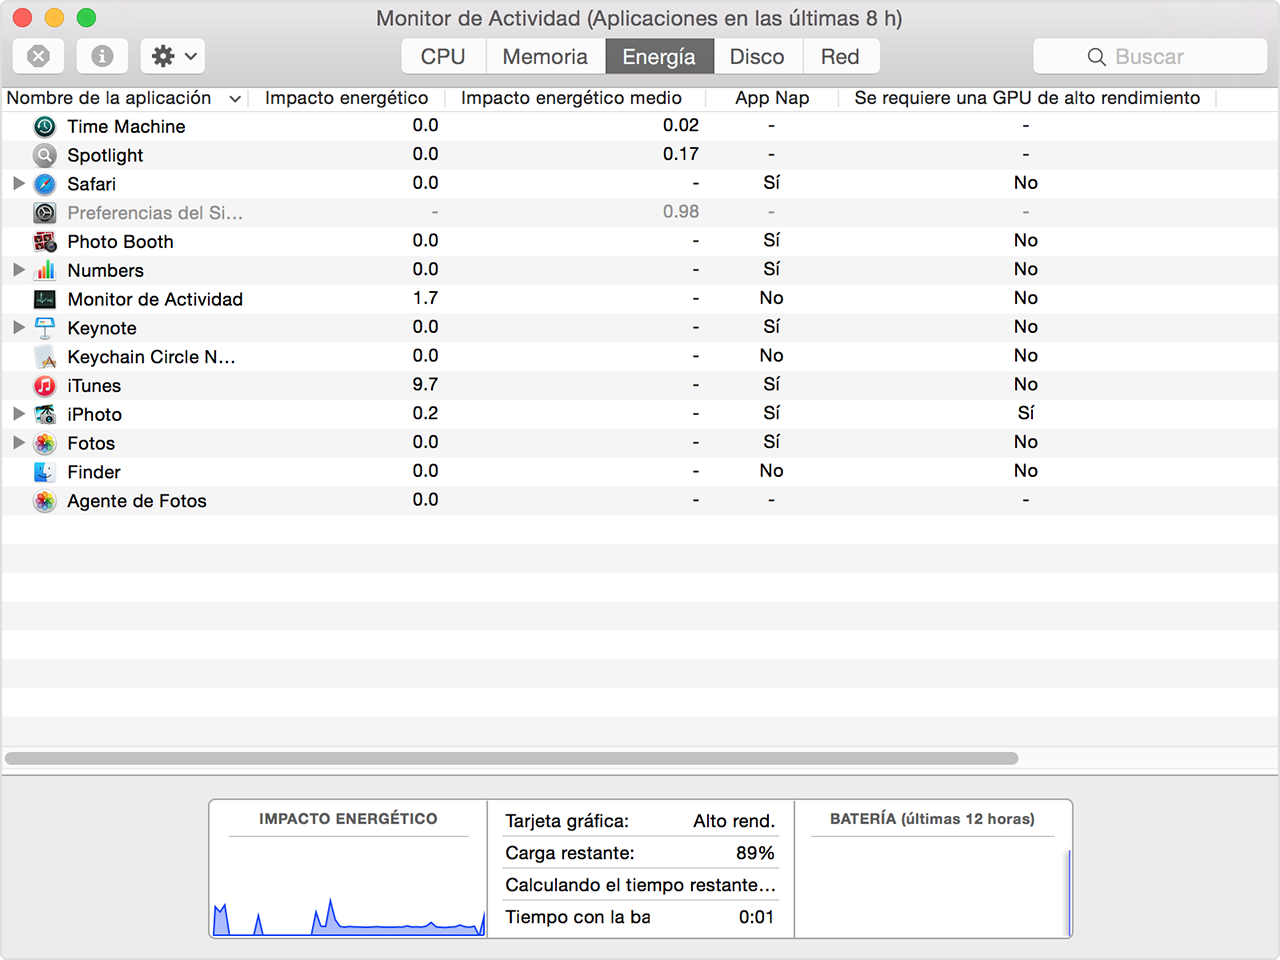
\includegraphics[width=1\textwidth]{03macActivityMonitorEnergy}
  \caption{Panel Energia}
  \label{fig:macActivityMonitorEnergy}
\end{figure}

En la parte inferior del panel Energía:

\begin{itemize}
  \item \textit{Impacto energético:} una medición relativa del total de energía utilizado por todas las apps.
  \item \textit{Tarjeta gráfica:} el tipo de tarjeta gráfica que se utiliza actualmente.
  \item \textit{Carga restante:} el porcentaje de carga restante de la batería de una Mac portátil.
  \item \textit{Tiempo para la carga completa:} la cantidad de tiempo que debe estar enchufada la Mac portátil a un tomacorriente de CA para cargarse por completo.
  \item \textit{Tiempo conectada:} el tiempo transcurrido desde que se enchufó la Mac portátil al tomacorriente de CA.
  \item \textit{Tiempo restante:} la cantidad estimada de tiempo restante de la batería en la Mac portátil.
  \item \textit{Tiempo con la batería:} el tiempo transcurrido desde que se desenchufó la Mac portátil del tomacorriente de CA.
  \item \textit{Batería (últimas 12 horas):} el nivel de carga de la batería de la Mac portátil durante las últimas 12 horas. El color verde muestra los momentos en que la Mac obtenía alimentación de un adaptador de energía.
\end{itemize}

\subsubsection{Disco}

El panel Disco muestra la cantidad de datos que cada proceso leyó del disco y escribió en el disco. También muestra las "lecturas entrantes" y las "escrituras salientes" (E/S), lo que representa la cantidad de veces que la Mac accede al disco para leer y escribir datos.

\begin{figure}[H]
  \centering
  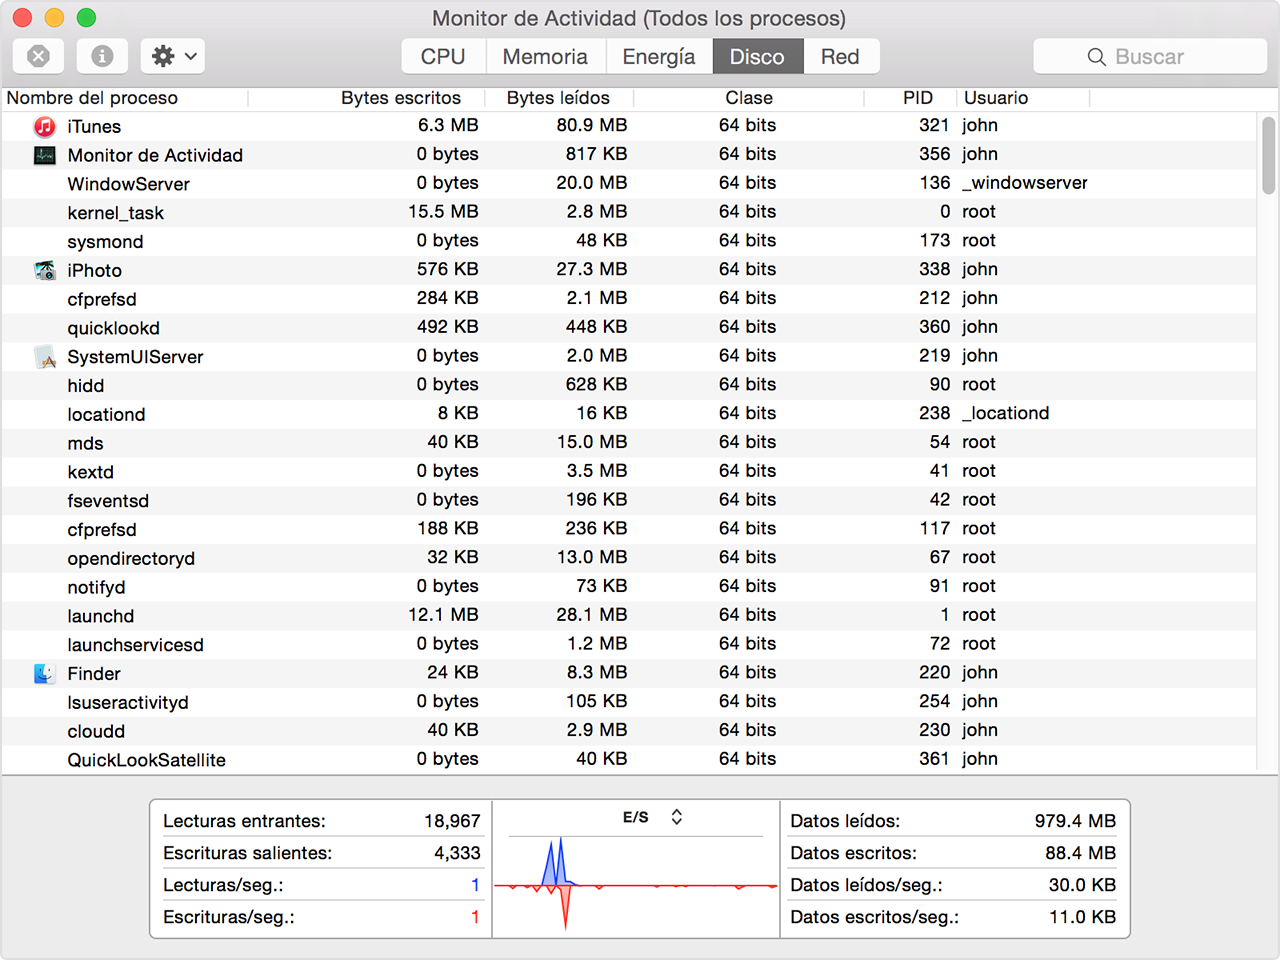
\includegraphics[width=1\textwidth]{04macActivityMonitorDisk}
  \caption{Panel Disco}
  \label{fig:macActivityMonitorDisk}
\end{figure}

La información en la parte inferior del panel Disco muestra la actividad total del disco en todos los procesos. El gráfico incluye un menú emergente para alternar entre mostrar la actividad de E/S o los datos como una unidad de medición. El color azul muestra la cantidad de lecturas por segundo o la cantidad de datos leídos por segundo. El color rojo muestra la cantidad de escrituras salientes por segundo o la cantidad de datos escritos por segundo.

\subsubsection{Red}

El panel Red muestra cuántos datos envía o recibe la Mac por medio de la red. Utiliza esta información para identificar qué procesos envían o reciben la mayor cantidad de datos.

\begin{figure}[H]
  \centering
  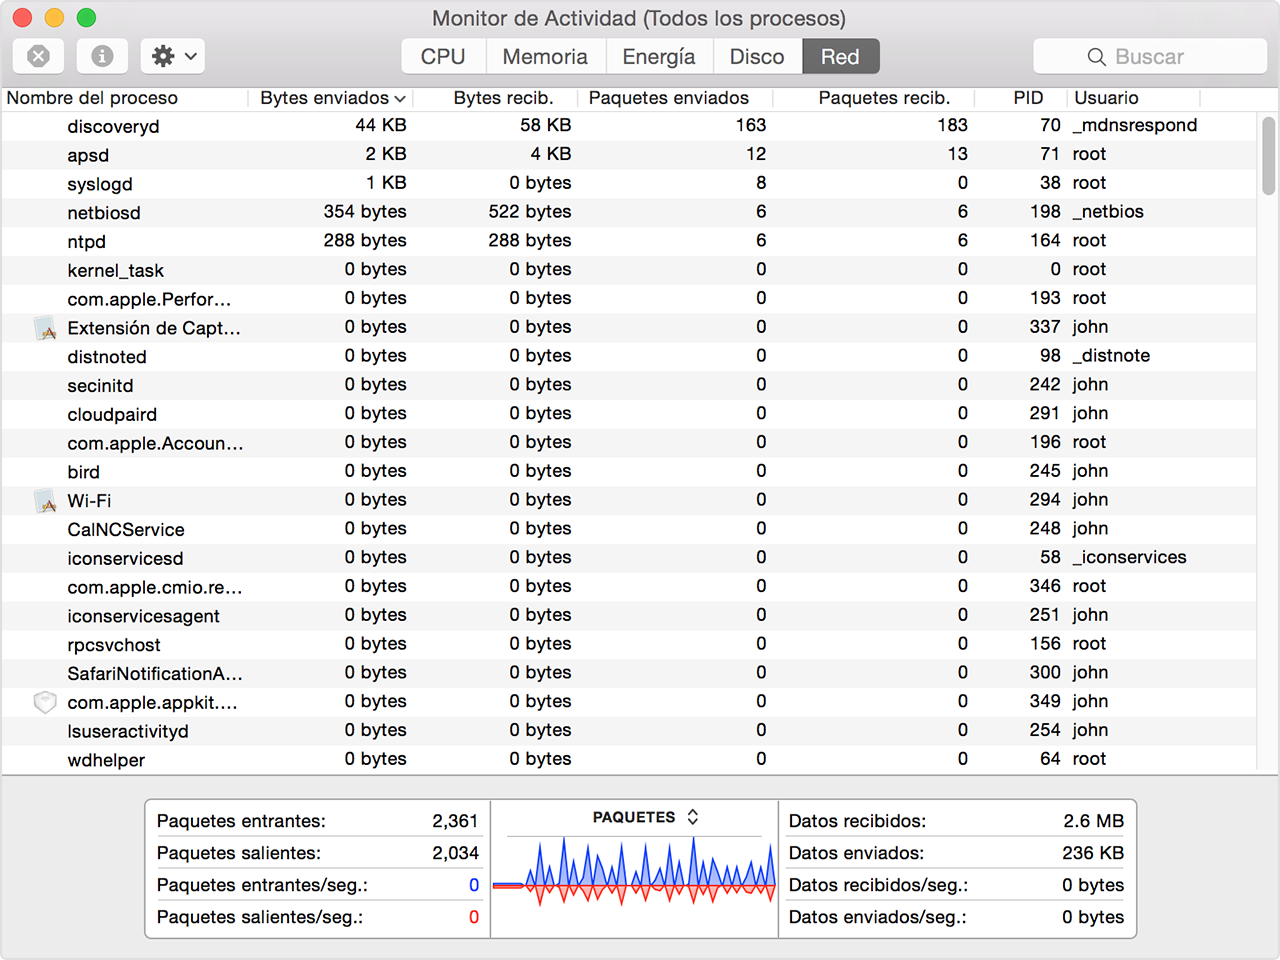
\includegraphics[width=1\textwidth]{05macActivityMonitorNetwork}
  \caption{Panel Red}
  \label{fig:macActivityMonitorNetwork}
\end{figure}

La información en la parte inferior del panel Red muestra la actividad total de red en todas las apps. El gráfico incluye un menú emergente para alternar entre mostrar paquetes o datos como una unidad de medición. El color azul muestra la cantidad de paquetes recibidos por segundo o la cantidad de datos recibidos por segundo. El color rojo muestra la cantidad de paquetes enviados por segundo o la cantidad de datos enviados por segundo.

\subsection{GNU/Linux}

\subsubsection{Monitor del Sistema}

 \cite{ref:web5} El Monitor del sistema en Linux es el interfaz gráfico de la orden top. Este interfaz viene instalado por defecto en la mayoría de las distribuciones. Si no estuviera, habría que instalarlo a través del paquete gnome-system-monitor, disponible en los repositorios oficiales.

La apariencia de este Monitor es muy similar al Administrador de tareas de Windows. Ofrece las siguientes opciones…

\begin{itemize}
  \item \textit{Sistema:} proporciona información básica como puede ser la versión del sistema operativo, el procesador integrado o la memoria RAM disponible.
  \item \textit{Procesos:} contiene un listado con los procesos del sistema, su estado y la carga media de los últimos minutos. También se puede crear un filtro para mostrar sólo determinados procesos, como pueden ser los procesos activos o los procesos del usuario. Sobre los procesos pueden realizarse varias operaciones como, por ejemplo, cambiar su prioridad, ver su mapa de memoria o finalizarlo (también denominado matarlo). Figura~\ref{fig:linuxMonitorSistemaProcesos}
  \item \textit{Recursos:} informa a través de gráficos dinámicos el uso de los principales recursos del sistema (el procesador, la memoria y la red). Es la forma más directa de monitorización. Esta pestaña permite ser personalizada. Figura~\ref{fig:linuxMonitorSistemaRecursos}
  \item \textit{Sistemas de archivos:} muestra un listado con los sistemas de archivos montados y sus principales características (espacio libre, punto de montaje, etc…). Figura~\ref{fig:linuxMonitorSistemaArchivos}
\end{itemize}

A través del Monitor del sistema no sólo se puede ejercer una monitorización de los principales elementos del sistema sino que también se puede modificar su comportamiento. Esto se hace aplicando una configuración directamente sobre el Monitor. La opción de configurar está disponible en el Monitor ejecutando la secuencia Editar -> Preferencias. Las preferencias hacen alusión principalmente a las pestañas de Procesos y Recursos, que son las que manejan los elementos más dinámicos.

\begin{figure}[H]
  \centering
  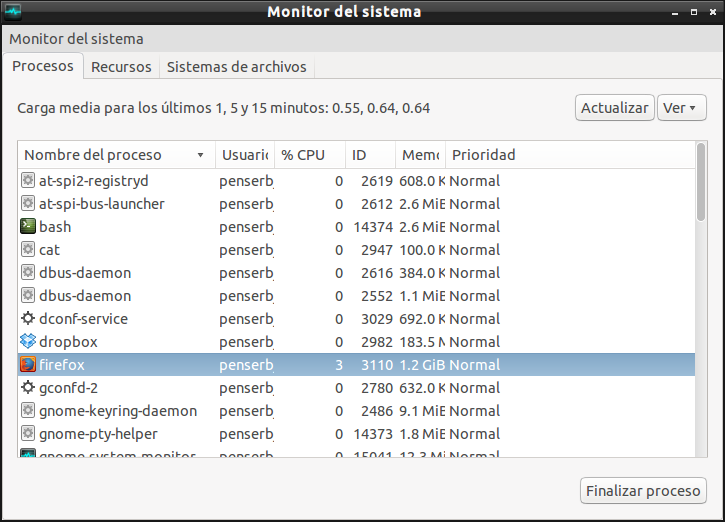
\includegraphics[width=1\textwidth]{06linuxMonitorSistemaProcesos}
  \caption{Panel Procesos}
  \label{fig:linuxMonitorSistemaProcesos}
\end{figure}

\begin{figure}[H]
  \centering
  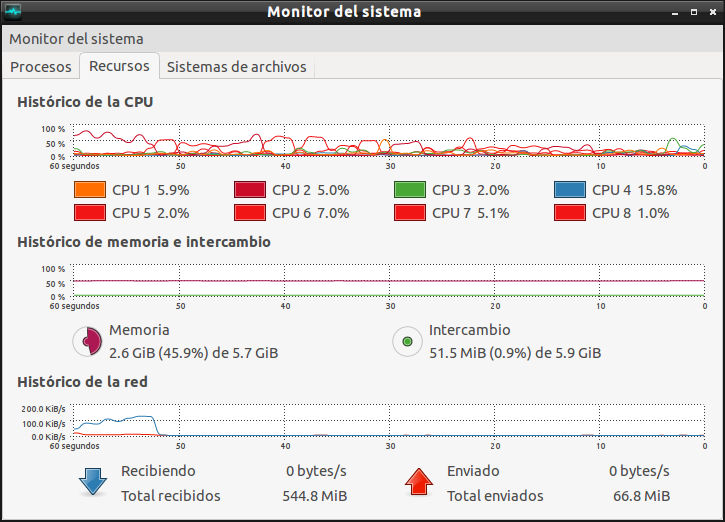
\includegraphics[width=1\textwidth]{07linuxMonitorSistemaRecursos}
  \caption{Panel Recursos}
  \label{fig:linuxMonitorSistemaRecursos}
\end{figure}

\begin{figure}[H]
  \centering
  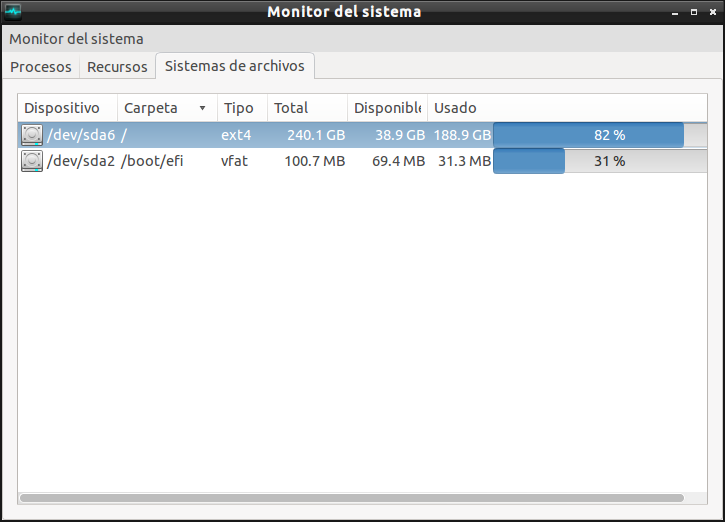
\includegraphics[width=1\textwidth]{08linuxMonitorSistemaArchivos}
  \caption{Panel Archivos}
  \label{fig:linuxMonitorSistemaArchivos}
\end{figure}

\subsubsection{Desde Terminal}

 \cite{ref:web6} A continuacion se muestra una lista con algunos de los comandos básicos que podremos utilizar en la terminal de cualquier distribución GNU/Linux para obtener información sobre nuestro sistema.

\begin{itemize}
  \item \textit{ps:} Imprime los procesos en ejecución y estadísticas asociadas..
  \item \textit{top:} Porcentaje y tiempo de CPU, así como uso de memoria, de procesos e hilos
  \item \textit{vmstat:} Utilización de la memoria virtual (VM) del sistema.
  \item \textit{free:} Consumo global de la VM.
  \item \textit{pmap:} Detalles de la VM de un proceso.
  \item \textit{netstat:} Muestra conexiones de red, tablas de enrutamiento, estadisticas sobre interfaces, entre otros.
  \item \textit{traceroute:} Imprime el trazo de los paquetes a través de los distinos nodos de red hacia un destino específico.
  \item \textit{ifconfig:} Detalla (también modifica) la configuración de las interfaces de red.
  \item \textit{df:} Uso del disco.
  \item \textit{lsof:} Lista archivos abiertos (incluidas las bibliotecas dinámicas) a nivel global o de un proceso determinado.
  \item \textit{fuser:} Identica los procesos que están usando un archivo o socket de red específico.
  \item \textit{stat:} Muestra el estado de un archivo, o de un sistema de archivos.
  \item \textit{who:} Lista quienes están logueados, y en qué terminales.
  \item \textit{w:} Igual al anterior, pero muestra que procesos están ejecutando.
  \item \textit{ulimit:} Muestra (o cambiá) los limites (stack, heap, procesos y archivos abiertos) de un usuario.
\end{itemize}


\section{Diseño}

\subsection{Propuesta de Monitor de Sistema}

\subsection{Diseño}

\section{Implementación}

\begin{thebibliography}{}

\bibitem{ref:web1}
  The GNOME Project.
  (-).
  Monitor del sistema.
  23/09/2016, 
  de The GNOME Project 
  Sitio web:   \url{https://help.gnome.org/users/gnome-system-monitor/index.html.es}

\bibitem{ref:web2}
  Xataka Winows. 
  (14/07/2014). 
  El administrador de tareas de Windows: qué es y cómo funciona. 
  23/09/2016, de Xataka Winows 
  Sitio web: \url{http://www.xatakawindows.com/bienvenidoawindows8/el-administrador-de-tareas-de-windows-que-es-y-como-funciona}

\bibitem{ref:web3}
  Arik Brooks. 
  (-). 
  Operating System and Process Monitoring Tools. 
  23/09/2016, de Washington University in St. Louis - School of Engineering \& Applied Science 
  Sitio web: \url{http://www.cs.wustl.edu/~jain/cse567-06/ftp/os_monitors/}

\bibitem{ref:web4}
  Apple. 
  (-). 
  Cómo usar Monitor de Actividad en la Mac. 
  23/09/2016, de Apple 
  Sitio web: \url{https://support.apple.com/es-mx/HT201464}

\bibitem{ref:web5}
  -. 
  (-). 
  Monitor del sistema. 
  25/09/2016, de Obasoft 
  Sitio web: \url{http://www.obasoft.es/CF/SIINF/SIINF_05_Contenidos/monitor_del_sistema.html}
  
\bibitem{ref:web6}
  Yúbal FM. 
  (01/10/2015). 
  Cómo monitorizar constantemente el rendimiento de tu distro GNU/Linux. 
  25/09/2016, de Genbeta 
  Sitio web: \url{http://www.genbeta.com/linux/como-monitorizar-constantemente-el-rendimiento-de-tu-distro-gnu-linux}

\end{thebibliography}

Biblioteca ncurses, C
\end{document}
